\documentclass[12pt]{article}
\usepackage[T2A,T1]{fontenc}
\usepackage[utf8]{inputenc}
\usepackage[english,russian]{babel}
\usepackage{adjustbox}
\usepackage{amsmath}
\usepackage{geometry}
\usepackage{wrapfig}
\usepackage{fancyhdr}

\usepackage{geometry}
\geometry{top=10mm}
\geometry{bottom=5mm}
\geometry{left=15mm}
\geometry{right=15mm}

\usepackage{graphicx}
\graphicspath{ {../images/} }
\usepackage{wrapfig}


\setlength{\parskip}{0pt}

\usepackage{fancyhdr}
\pagestyle{empty}
\begin{document}
\begin{center}
{\large
Федеральное государственное автономное образовательное учреждение\\
высшего образования\\
«Национальный исследовательский университет ИТМО»\\
\vspace{5pt}
Факультет программной инженерии и компьютерной техники\\
}
\vspace{17em}
{\Large Практическая работа №5} \Large по дисциплине\\
\smallskip
{\LARGE \textbf{Теория вероятностей и
математическая статистика}}\\[1em]
{\large Вариант №12}
\end{center}
\vspace{20em}
{\large
\begin{flushright}
Выполнил: Селянта Олег Дмитриевич\\
Группа: P3214\\
Преподаватель: Селина Елена Георгиевна\\
\end{flushright}
\vspace{\fill}
\begin{center}
Санкт-Петербург
2023г.
\end{center}
}\newpage
\smallskip
\textbf{\LARGE Задание}

\smallskip
\parindent=0mmКаждый студент получает выборку из 20 чисел. Необходимо определить следующие статистические характеристики: вариационный ряд, экстремальные значения и размах, оценки математического ожидания и среднеквадратического отклонения, эмпирическую функцию распределения и её график, гистограмму и полигон приведенных частот группированной выборки. Для расчета характеристик и построения графиков нужно написать программу на одном из языков программирования. Листинг программы и результаты работы должны быть представлены в отчете по практической работе\\
\textbf{\large Вариант №12}

\smallskip
\renewcommand{\arraystretch}{1.5}\begin{adjustbox}{max width=\textwidth}
\begin{tabular}{|c|c|c|c|c|c|c|c|c|c|c|c|c|c|c|c|c|c|c|c|}
\hline
{\large 0.41} & {\large 1.63} & {\large -1.53} & {\large -0.2} & {\large 0.85} & {\large 0.09} & {\large 1.54} & {\large 0.25} & {\large 1.24} & {\large -0.26} & {\large 1.08} & {\large 0.42} & {\large -0.92} & {\large -0.91} & {\large 1.15} & {\large -0.82} & {\large 0.26} & {\large 0.96} & {\large 1.57} & {\large 0.72}\\
\hline
\end{tabular}
\end{adjustbox}
\textbf{\LARGE Выполнение}

\smallskip
\textbf{\large Вариационный ряд}

\smallskip
\renewcommand{\arraystretch}{1.5}\begin{adjustbox}{max width=\textwidth}
\begin{tabular}{|c|c|c|c|c|c|c|c|c|c|c|c|c|c|c|c|c|c|c|c|}
\hline
{\large -1.53} & {\large -0.92} & {\large -0.91} & {\large -0.82} & {\large -0.26} & {\large -0.2} & {\large 0.09} & {\large 0.25} & {\large 0.26} & {\large 0.41} & {\large 0.42} & {\large 0.72} & {\large 0.85} & {\large 0.96} & {\large 1.08} & {\large 1.15} & {\large 1.24} & {\large 1.54} & {\large 1.57} & {\large 1.63}\\
\hline
\end{tabular}
\end{adjustbox}
\textbf{\large Статистический ряд}

\smallskip
\renewcommand{\arraystretch}{1.5}\begin{adjustbox}{max width=\textwidth}
\begin{tabular}{|c|c|c|c|c|c|c|c|c|c|c|c|c|c|c|c|c|c|c|c|}
\hline
{\large -1.53} & {\large -0.92} & {\large -0.91} & {\large -0.82} & {\large -0.26} & {\large -0.2} & {\large 0.09} & {\large 0.25} & {\large 0.26} & {\large 0.41} & {\large 0.42} & {\large 0.72} & {\large 0.85} & {\large 0.96} & {\large 1.08} & {\large 1.15} & {\large 1.24} & {\large 1.54} & {\large 1.57} & {\large 1.63}\\
\hline
{\large 1} & {\large 1} & {\large 1} & {\large 1} & {\large 1} & {\large 1} & {\large 1} & {\large 1} & {\large 1} & {\large 1} & {\large 1} & {\large 1} & {\large 1} & {\large 1} & {\large 1} & {\large 1} & {\large 1} & {\large 1} & {\large 1} & {\large 1}\\
\hline
\end{tabular}
\end{adjustbox}
\textbf{\large Экстремальные значения}

\smallskip
\parindent=0mmМинимальное значение: $x_{0}$ = -1.53; Максимальное значение: $x_{20}$ = 1.63\\
\textbf{\large Размах}

\smallskip
\parindent=0mmРазмах = наибольшее значение - наименьшее значение = $x_{20}$ - $x_{0}$; Размах = 3.16\\
\textbf{\large Математическое ожидание}

\smallskip
\parindent=0mmДля данной выборки статистический ряд будет совпадать с вариационным, так как каждое значение встречается только раз\\
\parindent=0mmВыборочное среднее (выборочное математическое ожидание) - среднее арифметическое всех значений выборки, считается по формуле: $$\overline{x_B} = \frac{1}{n} \sum_{i=1}^k x_i\cdot n_i$$\\
\parindent=0mmДля исходной выборки $$\overline{x_B} = 0.3765$$\\
\textbf{\large Выбороная дисперсия}

\smallskip
\parindent=0mm Выбороная дисперсия $D_B$ - среднее арифметическое квадратов отклонений значений выборки от выборочной средней $\overline{x_B}$, считается по формуле: $$D_B = \frac{1}{n} \sum_{i=1}^k (x_i - \overline{x_B})^2 \cdot n_i$$\\
\newpage
\parindent=0mmДля исходной выборки $$D_B = 0.3765$$\\
\textbf{\large Среднеквадратическое отклонение}

\smallskip
\parindent=0mm Выборочное среднее квадратическое отклонение выборки определяется формулой $$\sigma_B = \sqrt{D_B}$$\\
\parindent=0mmДля исходной выборки $$\sigma_B = 0.897927$$\\
\textbf{\large Исправленное выборочное среднее квадратическое отклонение}

\smallskip
\parindent=0mm При решении практических используется величина $$S^2 = \frac{n}{n - 1} \sum_{i=1}^k (x_i - \overline{x_B})^2 \cdot n_i = \frac{n}{n - 1}D_B$$ Которая называется \textit{исправленной выборочной дисперсией}\\
\parindent=0mm Величина $S = \sqrt{S^2}$ называется исправленным выборочным средним квадратическим отклонением\\
\parindent=0mmДля исходной выборки $$S = 0.921254$$\\
\textbf{\large Эмпирическая функция распределения}

\smallskip
\parindent=0mm Эмпирической (статистической) функцией распределения называется функция $F_n^x(x)$, определяющая для каждого значения $x$ частность события $\{X < x\}$: $$F_n^*(x) = p^*\{X < x\}$$\\
\parindent=0mmГде $p^x = \frac{{n_x}}{{n}}$ - отношение количесвта вариантов \{X < x\} к общему числу вариантов\\
Для исходной выборки $$F_n^*(x) = \begin{cases}
0 & \text{при } x < -1.53\\
0.05 & \text{при } -1.53\leq x < -0.92\\
0.1 & \text{при } -0.92\leq x < -0.91\\
0.15 & \text{при } -0.91\leq x < -0.82\\
0.2 & \text{при } -0.82\leq x < -0.26\\
0.25 & \text{при } -0.26\leq x < -0.2\\
0.3 & \text{при } -0.2\leq x < 0.09\\
0.35 & \text{при } 0.09\leq x < 0.25\\
0.4 & \text{при } 0.25\leq x < 0.26\\
0.45 & \text{при } 0.26\leq x < 0.41\\
0.5 & \text{при } 0.41\leq x < 0.42\\
0.55 & \text{при } 0.42\leq x < 0.72\\
0.6 & \text{при } 0.72\leq x < 0.85\\
0.65 & \text{при } 0.85\leq x < 0.96\\
0.7 & \text{при } 0.96\leq x < 1.08\\
0.75 & \text{при } 1.08\leq x < 1.15\\
0.8 & \text{при } 1.15\leq x < 1.24\\
0.85 & \text{при } 1.24\leq x < 1.54\\
0.9 & \text{при } 1.54\leq x < 1.57\\
0.95 & \text{при } 1.57\leq x < 1.63\\
1 & \text{при } x \geq 1.63
\end{cases}$$
\begin {figure}[h]\centering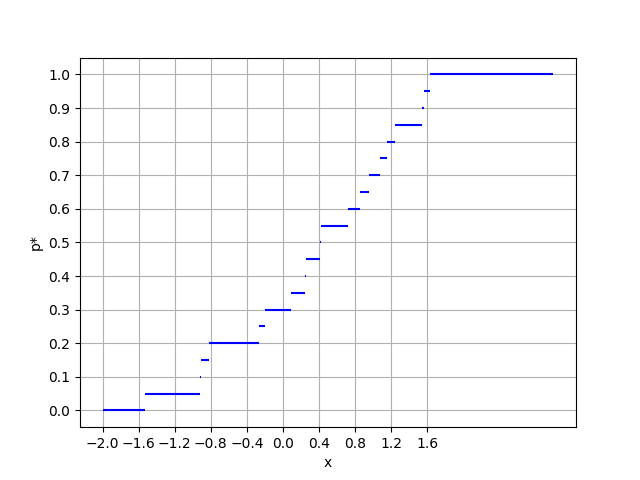
\includegraphics[width=0.8\textwidth]{./out/empirical_graph.png}\caption{График эмпирической функции распределения}\label{fig:my_label}\end{figure}
\newpage
\textbf{\large Интервальный статистический ряд}

\smallskip
\parindent=0mmТак как признак является непрерывным, то имеет смысл составить интервальный статический ряд (для дальнейшего использования в функции распределения). Пользуясь формулой Стерджеса, найдем величину интервала $$h = \frac{{x_{{max}} - x_{{min}}}}{{1 + log_2 n}}$$\\
\parindent=0mmДля исходной выборки $$h = 0.59377$$Учитывая рекомендацию по выбору начала первого интервала $x_{нач} = x_{min} - \frac{h}{2}$\\
\renewcommand{\arraystretch}{1.5}\begin{adjustbox}{max width=\textwidth}
\begin{tabular}{|c|c|c|c|c|c|}
\hline
{\large [-1.8269;-1.2331)} & {\large [-1.2331;-0.6393)} & {\large [-0.6393;-0.0456)} & {\large [-0.0456;0.5482)} & {\large [0.5482;1.142)} & {\large [1.142;1.7357)}\\
\hline
{\large 1} & {\large 3} & {\large 2} & {\large 5} & {\large 4} & {\large 5}\\
\hline
\end{tabular}
\end{adjustbox}
\begin {figure}[h]\centering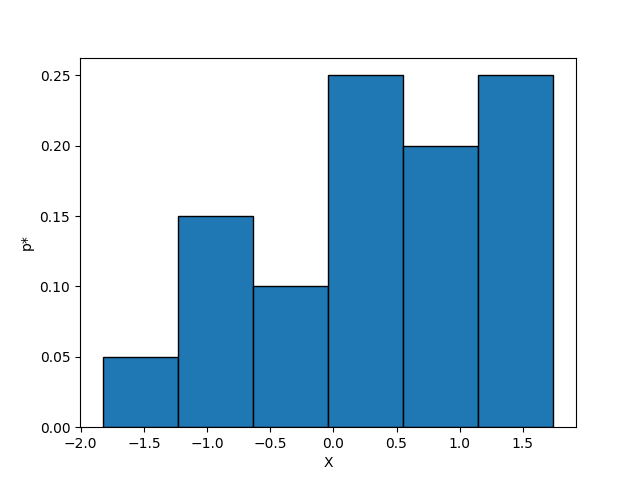
\includegraphics[width=0.8\textwidth]{./out/bar_char.png}\caption{Гистограмма}\label{fig:my_label}\end{figure}
\begin {figure}[t]\centering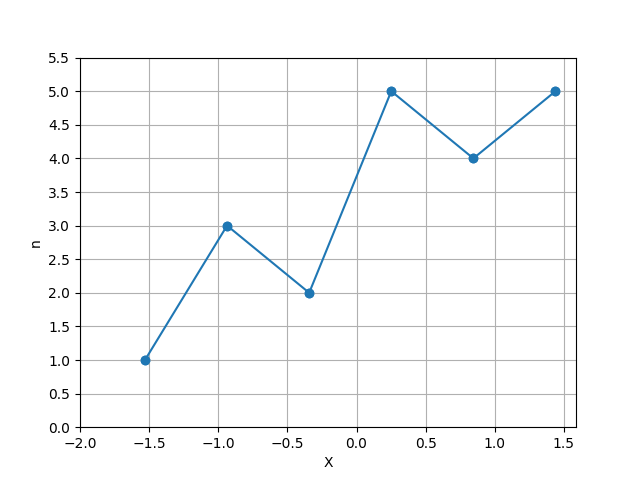
\includegraphics[width=0.8\textwidth]{./out/frequency_polygon.png}\caption{Полигон приведенных частот группированной выборки}\label{fig:my_label}\end{figure}
\end{document}